\subsection{Comparison Charts}

    \begin{figure}[h]
        \centering
        \captionsetup{justification=centering, margin=2cm}
        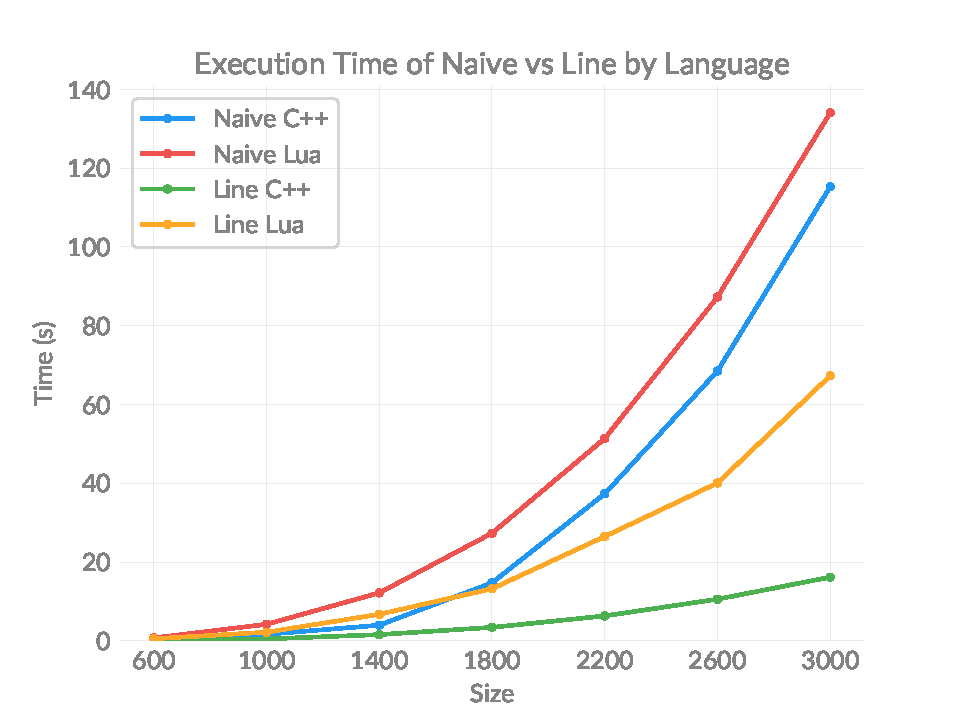
\includegraphics[width=0.8\textwidth]{pdf/naive-line-time}
        \caption{Time comparison between naive and line multiplication, in both C++ and Lua}
        \label{fig:chart:naive-line-time}
    \end{figure}

    \begin{figure}[h]
        \centering
        \captionsetup{justification=centering, margin=2cm}
        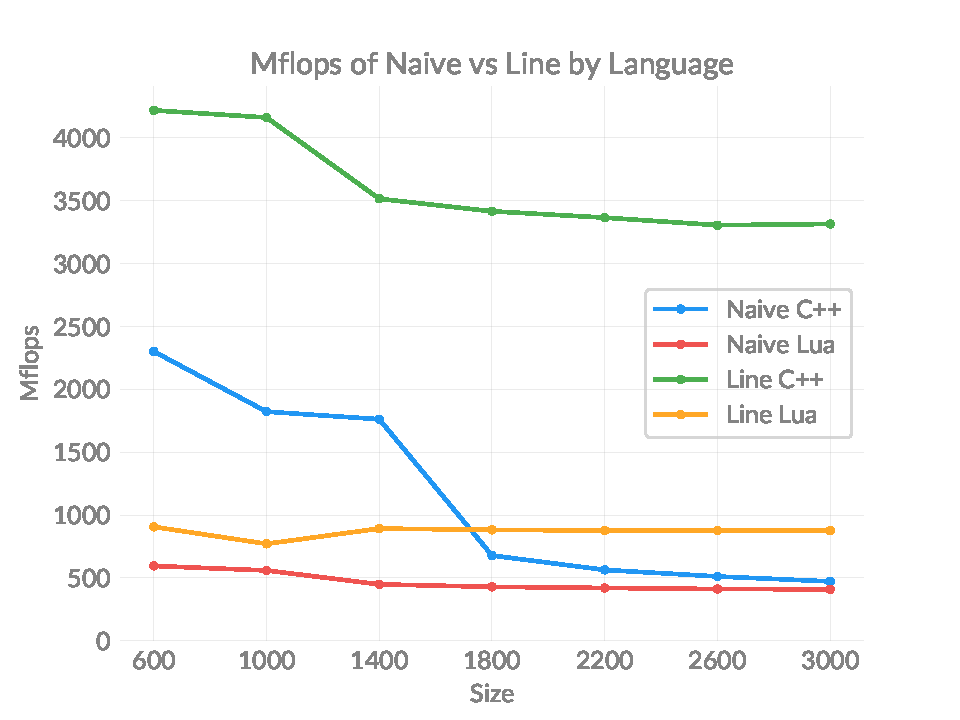
\includegraphics[width=0.8\textwidth]{pdf/naive-line-flops}
        \caption{Mflops comparison between naive and line multiplication, in both C++ and Lua}
        \label{fig:chart:naive-line-flops}
    \end{figure}

    \begin{figure}[h]
        \centering
        \captionsetup{justification=centering, margin=2cm}
        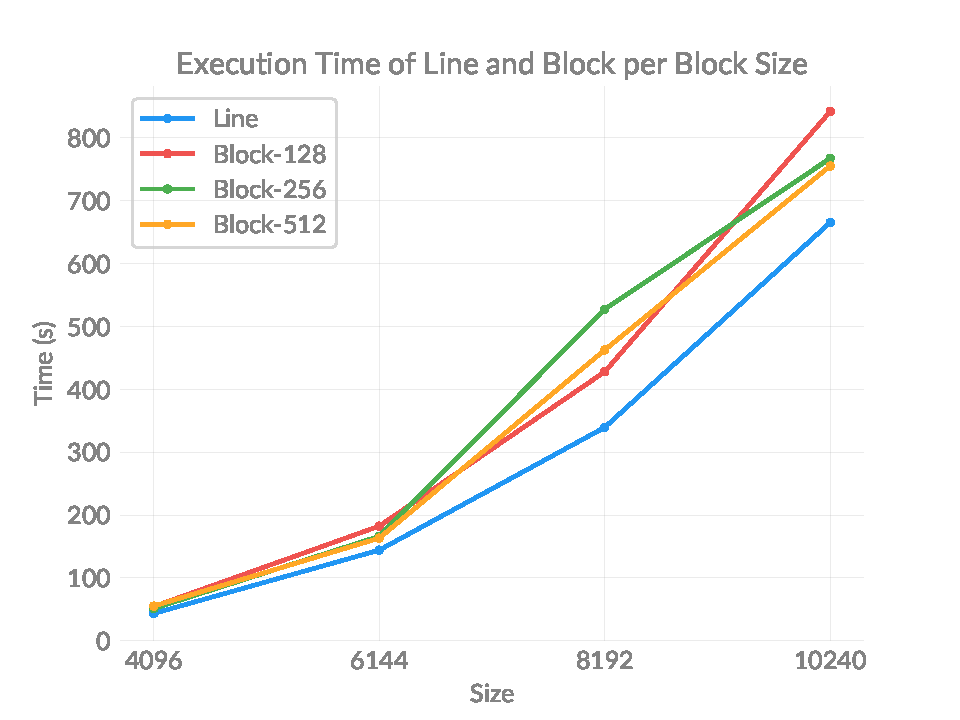
\includegraphics[width=0.8\textwidth]{pdf/line-block-time}
        \caption{Time comparison between line and block multiplication, with different block sizes}
        \label{fig:chart:line-block-time}
    \end{figure}

    \begin{figure}[h]
        \centering
        \captionsetup{justification=centering, margin=2cm}
        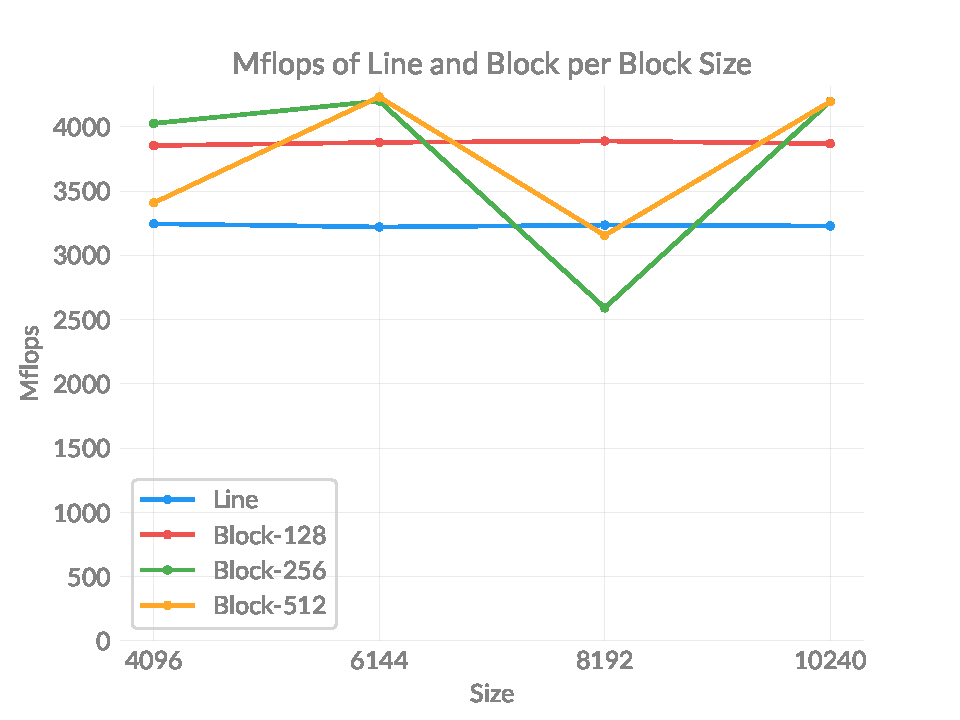
\includegraphics[width=0.8\textwidth]{pdf/line-block-flops}
        \caption{Mflops comparison between line and block multiplication, with different block sizes}
        \label{fig:chart:line-block-flops}
    \end{figure}

    \begin{figure}[h]
        \centering
        \captionsetup{justification=centering, margin=2cm}
        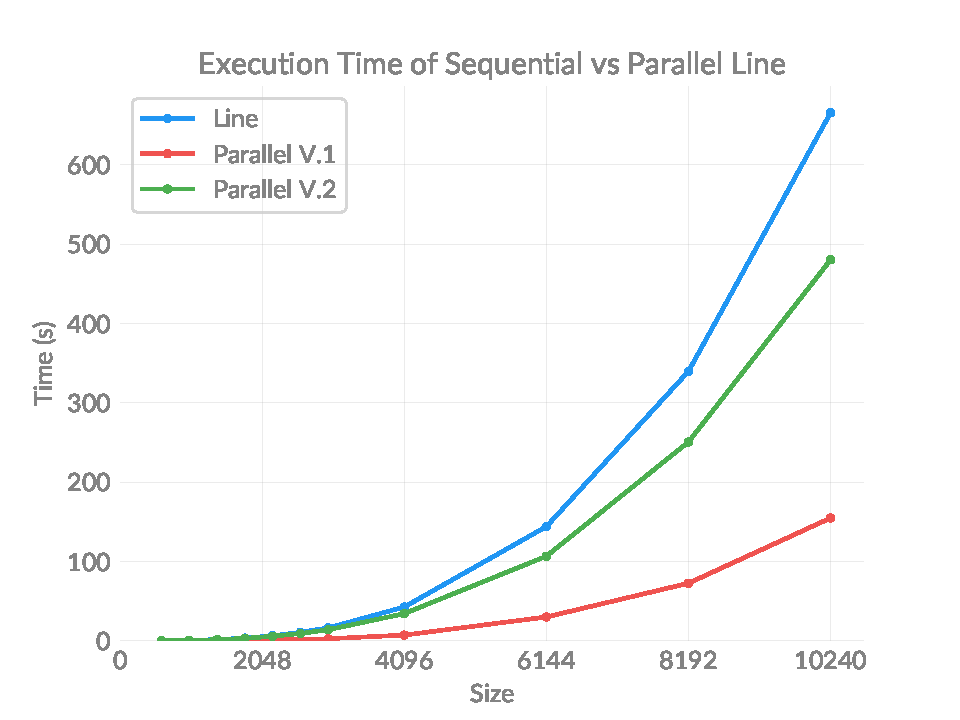
\includegraphics[width=0.8\textwidth]{pdf/parallel-time}
        \caption{Time comparison between sequential and parallel line multiplication}
        \label{fig:chart:parallel-time}
    \end{figure}

    \begin{figure}[h]
        \centering
        \captionsetup{justification=centering, margin=2cm}
        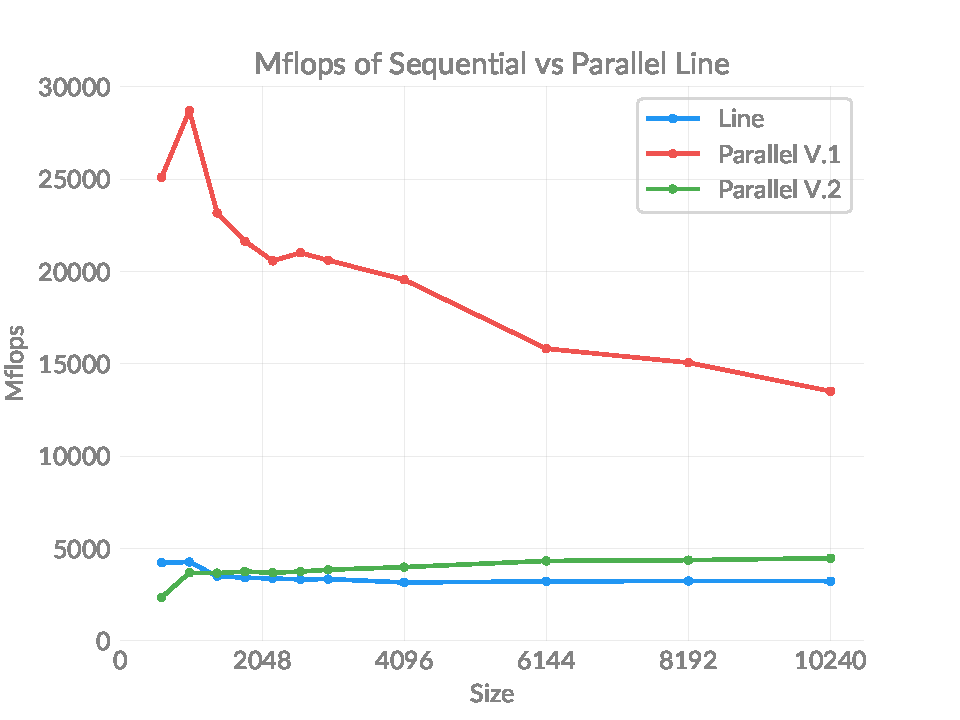
\includegraphics[width=0.8\textwidth]{pdf/parallel-flops}
        \caption{Mflops comparison between sequential and parallel line multiplication}
        \label{fig:chart:parallel-flops}
    \end{figure}

    \begin{figure}[h]
        \centering
        \captionsetup{justification=centering, margin=1.2cm}
        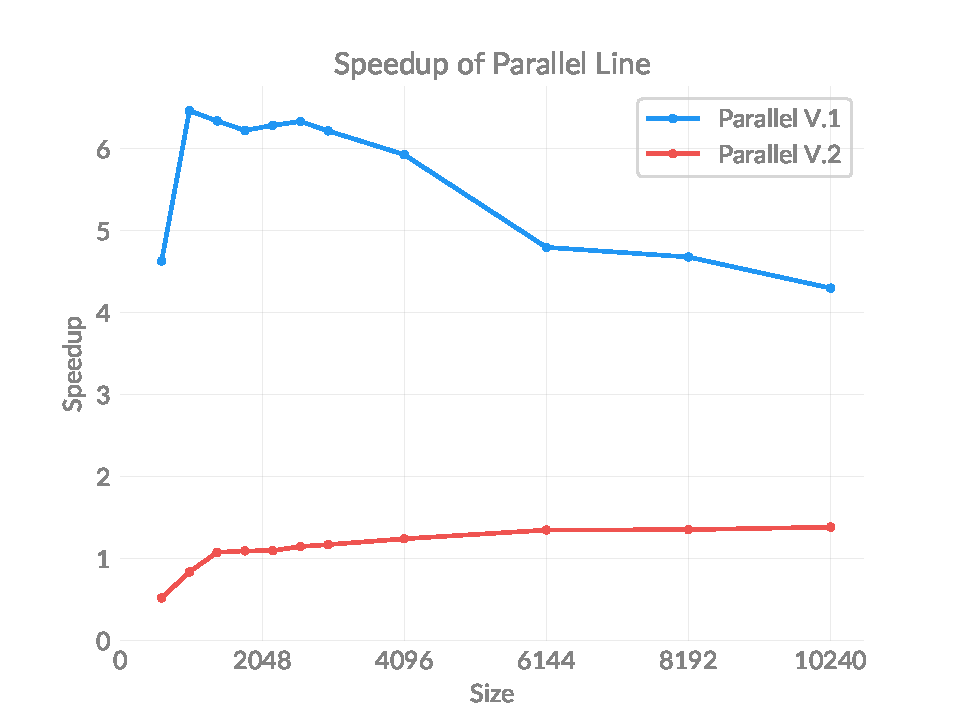
\includegraphics[width=0.8\textwidth]{pdf/parallel-speedup}
        \caption{Speedup comparison between versions of parallel line multiplication, relative to the sequential version}
        \label{fig:chart:parallel-speedup}
    \end{figure}

    \begin{figure}[h]
        \centering
        \captionsetup{justification=centering, margin=1.2cm}
        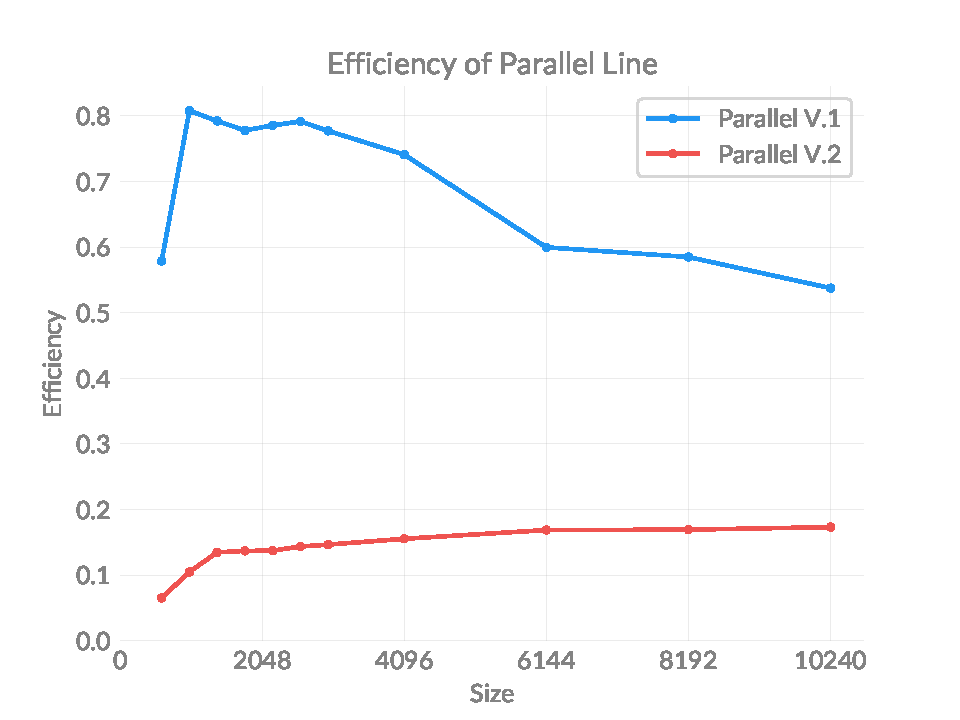
\includegraphics[width=0.8\textwidth]{pdf/parallel-efficiency}
        \caption{Efficiency comparison between versions of parallel line multiplication, relative to the sequential version}
        \label{fig:chart:parallel-efficiency}
    \end{figure}

\clearpage